\documentclass[letterpaper,11pt,twoside]{article}
\usepackage{amsmath,amssymb,amsfonts,amsthm}
\usepackage[margin=1.0in]{geometry}
\usepackage{fancyhdr, lastpage}
\usepackage[pdftex]{graphicx}
\usepackage{hyperref}
\hypersetup{
    colorlinks,
    citecolor={black},
    linkcolor={black},
    urlcolor={black},
    bookmarksnumbered,
    pdfstartview={FitH},
    pdfpagemode={UseOutlines},
    pdftitle={Project Report - Distributed Query Processing},
    pdfauthor={Larry Bowers, James Bradwell, Evan Dickinson, Bhadresh Patel, and Lewis Pearson},
    pdfsubject={CS 453 Project Report}
}

\setlength{\parskip}{0.5ex}
\pagestyle{fancy}
\setlength{\headheight}{14.0pt}
\fancyhead{}
\fancyfoot{}
\fancyhead[RO,RE] {Project Report: \emph{Distributed Query Processing}}
\fancyfoot[LO,LE] {CS 453: Project 4}
\fancyfoot[RO,RE] {Page \thepage\ of \pageref{LastPage}}
\renewcommand{\headrulewidth}{0.5pt}
\renewcommand{\footrulewidth}{0.5pt}

\begin{document}

%%%%%%%%%% Title Page %%%%%%%%%%%%%%%%%%%%%%%%%%%%%%%%%%%%%%%%%%%%%%%%%%%%%%%%%%
\begin{titlepage}
   \begin{center}
       {\Large \textbf{Project Report}}\\[0.5cm]
       {\Large \textbf{CS 453: Project 4}}\\[3.0cm]

       {\rule{\linewidth}{0.5mm}} \\[0.5cm]
       {\Huge \textbf{Distributed Query Processing}}\\[0.4cm] 
       {\rule{\linewidth}{0.5mm}} \\[2.0cm]

       \textbf{Larry Bowers}\\
       \texttt{killergift@wsu.edu}\\[0.5cm]
       \textbf{James Bradwell}\\
       \texttt{jebradwell@gmail.com}\\[0.5cm]
       \textbf{Evan Dickinson}\\
       \texttt{evan13579b@wsu.edu}\\[0.5cm]
       \textbf{Bhadresh Patel}\\
       \texttt{bhadresh@wsu.edu}\\[0.5cm]
       \textbf{Lewis Pearson}\\
       \texttt{lewis\_pearson@wsu.edu}\\[0.5cm]

       \vfill
       Washington State University Vancouver\\
       December 05, 2010
   \end{center}
\end{titlepage}

\begin{abstract}
The main goal of this project is to implement the user interface and the distributed query processing component of the Search Engine over multiple Amazon EC2 nodes using the PageRank and Indexes generated by previous project.
\end{abstract}

\section{Overview}

\begin{figure}[htbp]
 \centering
 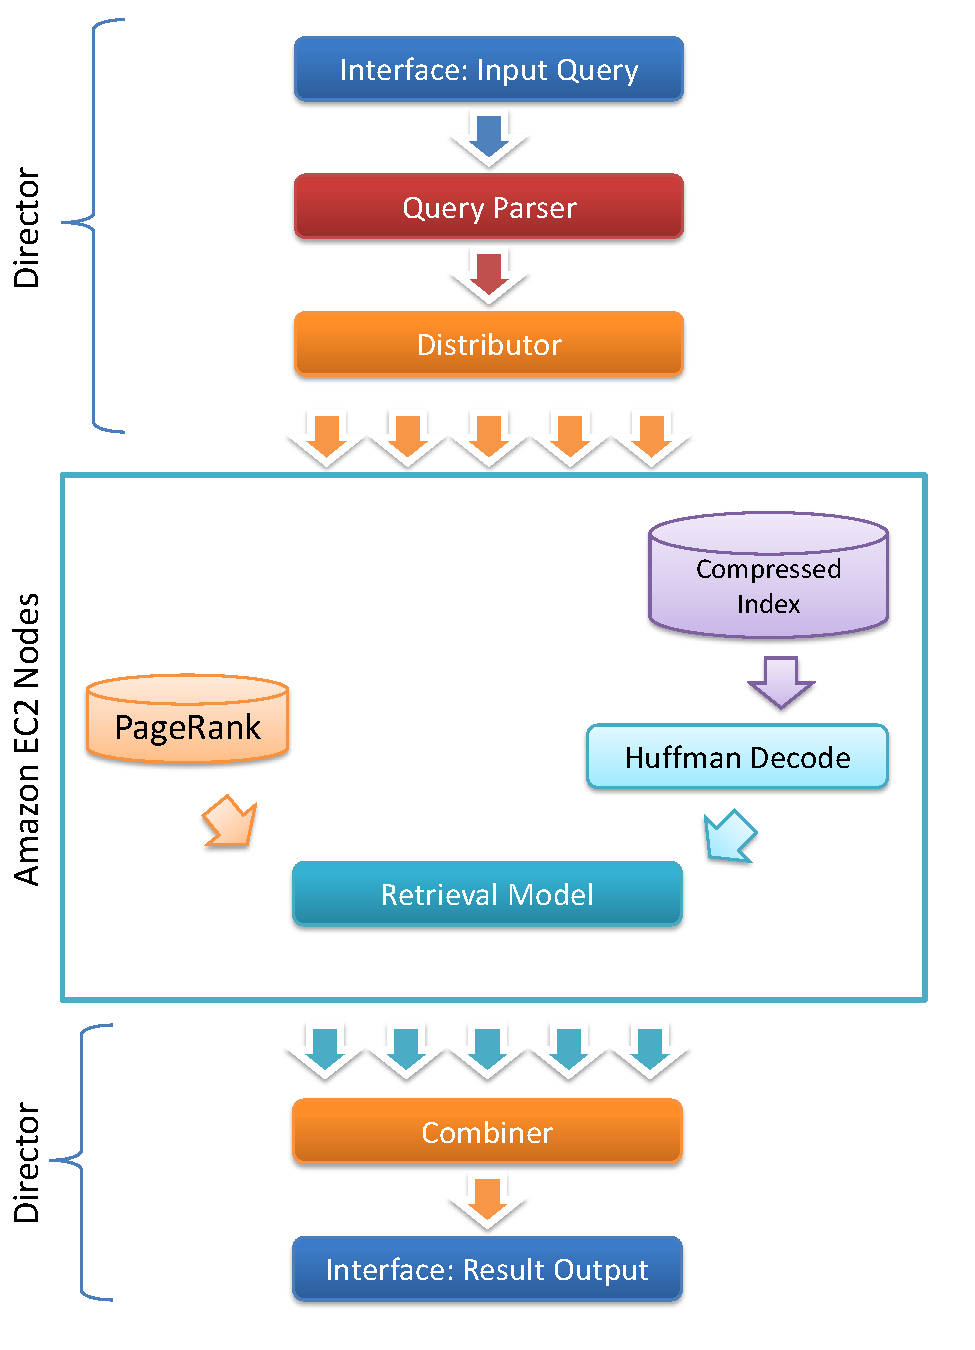
\includegraphics[trim=0.0in 0.00in 0.0in 0.0in, clip, page=1]{Architecture.pdf}
 \caption{Architecture Overview}
 \label{fig:Architecture}
\end{figure}

In this project, our goal is to implement distributed query processing component of the search engine. In previous projects, we already crawled documents, generated indexes, and calculated PageRank. Distributed query processing component utilities these information and perform user's query evaluation over multiple nodes. Figure~\ref{fig:Architecture} shows  architecture for distributed query processing. The user interface takes query input from the user and sends to the query parser. Query parser validates and parses the given query and hand off to distributer. Distributer, then connects to each index server and executes the given query. Index server finds ranked document list for the given query and sends back to distributer. Distributer merges the retrieved results and sends to the user interface, which is then displayed to the user.  

\section{Interface}

The projects UI was done with HTML, CSS and PHP script. The large and small search button and icon images were done in paint.net. There are two search pages as described in following sub sections. 

\subsection{Home Page}
The home page\footnote{http://ec2-174-129-159-24.compute-1.amazonaws.com/ui/} is very simple. It has a nice splash page image and the search textbox with the search button centered underneath. Figure~\ref{fig:home_page} shows the home page.

\begin{figure}[htbp]
 \centering
 \includegraphics[trim=0.0in 5.35in 0.0in 0.0in, clip, page=2]{Architecture.pdf}
 \caption{Home Page}
 \label{fig:home_page}
\end{figure}

\subsection{Results Page} 
The results page may be accessed by entering in a query into the search box on the home page. Figure~\ref{fig:result_page} shows the sample result page when the search is done for a query `test'.

\begin{figure}[htbp]
 \centering
 \includegraphics[trim=0.0in 1.75in 0.0in 0.0in, clip, page=3]{Architecture.pdf}
 \caption{Results Page}
 \label{fig:result_page}
\end{figure}

The pages use a style much like Google’s layout to create a similar feel for users familiar with the Google search pages. The results page displays the navigation links. There are ten links per pagination. There are only ten pagination links displayed at any given time. From the current pagination link five pagination links are displayed to the left and four are displayed to the right. Each retrieved entry has the following: Title of the page linked with its actual URL, Page Rank with its current page rank, Score with it current score and then the actual URL with a Cached link to our locally saved version of the file. The retrieval time and result count are displayed under the search textbox. To return back to the first page with just the search text box you may click on the small icon to the left of the search box on the results page. Some challenges with the UI were working with PHP and retrieving data sent back from the cloud. Being only moderately familiar with PHP there was a bit of a learning curve. Bhadresh had helped tremendously with the PHP code and validating my PHP code. 

\section{Query Parser}
The grammar listed in the project requirements deemed unfit by Lewis and I. We decided the grammar would be more usable/easier if spaces were set as OR and strictly used `+' as AND's, thus the grammar changed to this.
\begin{align*}
	Q &:: = expr \\
	expr &:: = \epsilon \, | \, \tau \, expr \\
	\tau &:: = s[a-zA-Z0-9]\backslash w \\
	s &:: = \epsilon \, | - | + | \backslash w
\end{align*}
These changes makes sure there is only one `term decider' (\textbackslash w,-,+) before each term and whitespace directly after each term, there is one exception with the query, the first term typically will not have a `term decider'. If one does not exist it will default to OR.  

The new grammar rules require that the query be tested for terms directly following a `term decider'. A term must begin with an alpha character, for example a term `34jk' will be rejected and the query will not be valid.

The Parser uses the same Stopper/Stemmer from project 2 of team1’s project solution. The stopping list is from onjava.com site\footnote{http://onjava.com/onjava/2003/01/15/examples/EnglishStopWords.txt}. The stemming code is based off the original paper Porter, 1980, An algorithm for suffix stripping, Program, Vol. 14, no. 3, pp 130-137\footnote{http://www.tartarus.org/~martin/PorterStemmer}. To ensure correctness of the 3rd party implementation I tested the algorithm’s input/output against a long dictionary of words found on the algorithm's site.

\subsection{Challenges}
Considering this is the second time using python I struggled with syntax mostly. Another challenge was making sure that the two porter stemmer algorithms (C\# version from project 2 and the python version) had the same output for any input. Other the coding issues the group seemed to work very well together and everyone completed their part of the project.


\section{Distributed Evaluation}

The distributed evaluation is done using six Amazon EC2 nodes as shown in figure~\ref{fig:Architecture}. One of the nodes is called director, that is responsible for hosting the user interface, execute search on all index server, combine the results, and then return the ranked list of documents to user interface. Processing of the query given by the user interface is done in simple client-server model, where index server is a simple daemon process that is started once and the distributer is client that connects to each index server when query is executed.

\subsection{Index Server}

The index server is a simple daemon process that is started and listens on socket for incoming query request. When the index server is started it load various information into the memory first and then waits for the incoming request. It loads PageRank, Index file, and pid\_map.dat files during initialization. The startup process takes indexfile name as an argument; \emph{i.e.}, which index file to use on the particular node. Thus, for each query request it only calls retrieval model to calculate relevance score using pre-loaded information in the memory. The query request contains two information: (i) Retrieval Model to use, and (ii) parsed and validated user's query. Based on the given retrieval model, index server calls the appropriate model's code to get ranked list of documents. Once the results are retrieved, they are sent back to the distributor. 

\subsection{Distributer}

Distributer is a client program, that connects to each index server, sends the query given by the user interface. It then waits for the results, collects results form all index servers and merge them. The merged results are then sorted based on relevance score and sent back to the UI based on the requested page number. Distributer creates multiple processes or threads to connect to each index server, thus it executes queries in parallel on each index server. 

Based on the query terms, distributer first finds which index server needs to be called. Since index files are sorted and split across index servers, any particular term would be available one index server only. This way we can optimize for number of processes distributer needs to create and avoid unnecessary search to any index server. 

\section{Index Compression}

\subsection{Huffman Encoding}
The first decision our group made about this feature is whether or not to consider each doc number as an atom or each character. We chose characters as atoms for simplicity and because we were unsure about how choosing numbers as atoms would scale.

To facilitate huffman encoding a class was created that stored the information needed to encode and decode for a particular document set. The class also had the methods needed to do the encoding and decoding.

To set up huffman encoding, the index files were stripped of all the terms plus the first separator because the terms were not to be encoded.

A code was then created with createCode.py on the stripped index files to get a proper encoding for the document set.

The result of creating the code was a huffman coder object that had the data and methods needed to encode and decode that document set. The object was pickled and saved into a file called `huffmanCode'.

The index files were then processed into maps and pickled. Two maps were created for each index, one that had compressed values and the other non-compressed. The maps were actually maps of maps where the first level had a `type' key saying whether the data was compressed or uncompressed and a `data' key whose corresponding value was a map containing all the terms with the string that contains their counts information.

The compressed index had to be pickled so that the count string wouldn't create ambiguities when compressed into a binary form. If the terms were not separated from the compressed count string the compressed count string could have been compressed into a newline followed by what looks like a term making one think that the part that is compressed follows the illusionary newline and false-term.

Since the compressed index had to be pickled, the normal one was also pickled for consistency and also so that the pickled map could hold information about whether or not it was compressed.

Example index:
ant:4:(434,1)

ant becomes key with corresponding value: \texttt{4:(434,1)} in non-compressed version and \texttt{\#\$\^\$} in compressed version.

\subsection{Huffman Decoding}
The retrieval model class contains a `coder' member which is read into the class from the `huffmanCode' file in the data directory at initialization.

This coder member is stored and sent to the score calculation functions to be used when retrieving term counts. The score calculation functions pass the coder to the getTermContent function which returns the terms based on the index type. The index is also passed to the getTermContent function and its `type' key is used to identify if it is compressed or not. If it is compressed the compressed count string is decompressed using the coder and the resulting decompressed string is then parsed into a map containing the counts for the term overall and in each document.

If the type of the index is `uncompressed' the index will have already had its count string parsed into an appropriate map which is returned by getTermContent.

The compression ratio for each count string was generally a little under 2.

For index-0 the size in memory of each map was ~460000 bytes compressed and ~740000 non-compressed (before each non-compressed entry is parsed into a map after which the non-compressed size would be much larger). The original file size was ~570000 bytes.

Time-wise no significant time increase was noticed. To test the time taking by decoding I ran a test that decoded the value corresponding to every term in the index and for 2500 files the result was 4 seconds.

4/2500=~1.6ms. Our average query was around 0.3 seconds or 300 ms making the decoding insignificant in comparison.

\section{Retrieval Model}

The retrieval model is responsible for determining relevance scores for use in page rankings. We have structured it by creating a module with a class that accepts a query, calls the appropriate retrieval model, and returns the results. We have implemented both the BM25 and Query Likelihood retrieval models.

The retrieval.py module contains the RetrievalModel class which is used to accept a query and return the associated relevance scores and document information. In the process of calculating relevance scores and finding associated document information, it is necessary to have access to the PID map, pageRank scores, and document term counts for all documents in the collection. Therefore, files containing this information are created and stored on the server prior to running the server. Upon instantiation, the RetrievalModel object reads and stores this information into memory, and stays active for the duration of the node's operation. All information is stored in dictionaries to minimize access times.

\subsection{Query Likelihood}
The Query Likelihood model's score calculation contains the constant \(\lambda\). We chose a default value of 0.1, which is best for short queries. The formula we used is:
\[
log P(Q|D)=\sum_{i=1}^{n}log((1-\lambda)\frac{f_{qi,D}}{|D|}+\lambda\frac{c_{q_{i}}}{|C|})
\]
where \(|D|\) is the number of words in the document, \(f_{qi,D}\) is the number of times word qi occurs in the document, \(c_{q_{i}}\) is the number of times word \(q_{i}\) occurs in the collection of documents, and \(|C|\) is the total number of terms in the collection of documents.

\subsection{BM25}
The BM25 model's score calculation contains the constants \(k_{1}\), \(k_{2}\), and b. The default values we have chosen for them are based on the textbook's recommendations and example. The formula we used for the BM25 model is:
\[
BM25(Q,D)=\sum_{i \in Q}log\frac{N-n_{i}+0.5}{n_{i}+0.5}\cdot \frac{(k_{1}+1)f_{i}}{K+f_{i}}\cdot \frac{(k_{2}+1)qf_{i}}{k_{2}+qf_{i}}
\]
where N is the total number of documents in the collection, \(n_{i}\) is the number of documents containing term i, \(f_{i}\) is the frequency of term i in the document, and \(qf_{i}\) is the frequency of term i in the query. The constants \(k_{1}\) and \(k_{2}\) are set to 1.2 and 100, respectively. The remaining term K is calculated as:
\[
K=k_{1}((1-b)+b\cdot \frac{|D|}{avDL})
\]
where \(|D|\) is the number of terms in the document, avDL is the average number of terms per document in the collection, and the constant b is set to 0.75.

\subsection{Summary}
Once all scores have been calculated, the pageRank scores are incorporated. In the case of BM25 scores, the pageRank is simply multiplied against the score. For Query Likelihood scores, we take the log of the associated pageRank value and add the two scores together.

We chose to use the Query Likelihood model as the default model. However, the two models actually return fairly similar results, and the textbook also mentions that the Query Likelihood model has been shown to be at least as effective as the BM25 algorithm. The choice was arbitrary. The use of BM25 is still available for any query.

\section{Roles}
\begin{description}
  \item[Larry Bowers] Query parser
  \item[James Bradwell] User interface
  \item[Evan Dickinson] Huffman encoding/decoding 
  \item[Bhadresh Patel] Distributed evaluation
  \item[Lewis Pearson] Retrieval model
\end{description}

\section{Test Environment}

For testing/production purpose, we have set up instances on Amazon EC2. The instance id of the director machine is i-5135773c which also hosts the user interface. Instance ids of five index servers are: (i) i-5335773e, (ii) i-2d357740, (iii) i-2f357742, (iv) i-29357744, and (v) i-2b357746. The source code on all instances is checked out at /home/ubuntu/dqp/. The user interface can be accessed via public DNS name of the director instance. For example, http://ec2-174-129-159-24.compute-1.amazonaws.com/ui/.

\section{Usage Guide}

\begin{itemize}
	\item Update Nodes file \texttt{dp/local.nodes} or \texttt{dp/cloud.nodes}. Change the IP address of all nodes for the appropriate environment.
	\item Start index server on each instance
\begin{verbatim}
	$ python ~/dqp/dp/server.py
\end{verbatim}
	\item Find the public DNS of the director instance \texttt{i-5135773c}. Launch the UI using public DNS, for example, http://ec2-174-129-159-24.compute-1.amazonaws.com/ui/.
\end{itemize}

\end{document}
